%%%%%%%% ICML 2019 EXAMPLE LATEX SUBMISSION FILE %%%%%%%%%%%%%%%%%

\documentclass{article}

% Recommended, but optional, packages for figures and better typesetting:
\usepackage{microtype}
\usepackage{graphicx}
\usepackage{subfigure}
\usepackage{booktabs} % for professional tables

\usepackage{amsmath}    
\usepackage{amssymb}  
\usepackage{multirow}
\usepackage{placeins}
\usepackage{graphbox}
\usepackage{caption}

% hyperref makes hyperlinks in the resulting PDF.
% If your build breaks (sometimes temporarily if a hyperlink spans a page)
% please comment out the following usepackage line and replace
% \usepackage{icml2019} with \usepackage[nohyperref]{icml2019} above.
\usepackage{hyperref}

% Attempt to make hyperref and algorithmic work together better:
\newcommand{\theHalgorithm}{\arabic{algorithm}}


\DeclareMathOperator\arctanh{arctanh}
\DeclareMathOperator\softmax{softmax}


% Use the following line for the initial blind version submitted for review:
\usepackage[accepted]{icml2019}

% If accepted, instead use the following line for the camera-ready submission:
%\usepackage[accepted]{icml2019}

% The \icmltitle you define below is probably too long as a header.
% Therefore, a short form for the running title is supplied here:
\icmltitlerunning{On the Vulnerability of Capsule Networks to Adversarial Attacks}

\begin{document}
\twocolumn[
\icmltitle{On the Vulnerability of Capsule Networks to Adversarial Attacks}

% It is OKAY to include author information, even for blind
% submissions: the style file will automatically remove it for you
% unless you've provided the [accepted] option to the icml2019
% package.

% List of affiliations: The first argument should be a (short)
% identifier you will use later to specify author affiliations
% Academic affiliations should list Department, University, City, Region, Country
% Industry affiliations should list Company, City, Region, Country

% You can specify symbols, otherwise they are numbered in order.
% Ideally, you should not use this facility. Affiliations will be numbered
% in order of appearance and this is the preferred way.
\icmlsetsymbol{equal}{*}

\begin{icmlauthorlist}
\icmlauthor{Felix Michels}{equal,hhu}
\icmlauthor{Tobias Uelwer}{equal,hhu}
\icmlauthor{Eric Upschulte}{equal,fzj}
\icmlauthor{Stefan Harmeling}{hhu}
\end{icmlauthorlist}

\icmlaffiliation{hhu}{Department of Computer Science, Heinrich-Heine-Universit\"at, D\"usseldorf, Germany}
\icmlaffiliation{fzj}{Institute of Neuroscience and Medicine INM-1, Forschungszentrum J\"ulich, J\"ulich, Germany}

\icmlcorrespondingauthor{Felix Michels}{felix.michels@hhu.de}
\icmlcorrespondingauthor{Tobias Uelwer}{tobias.uelwer@hhu.de}
% You may provide any keywords that you
% find helpful for describing your paper; these are used to populate
% the "keywords" metadata in the PDF but will not be shown in the document
\icmlkeywords{Adversarial Examples, Capsule Networks}

\vskip 0.3in
]

% this must go after the closing bracket ] following \twocolumn[ ...

% This command actually creates the footnote in the first column
% listing the affiliations and the copyright notice.
% The command takes one argument, which is text to display at the start of the footnote.
% The \icmlEqualContribution command is standard text for equal contribution.
% Remove it (just {}) if you do not need this facility.

%\printAffiliationsAndNotice{}  % leave blank if no need to mention equal contribution
\printAffiliationsAndNotice{\icmlEqualContribution} % otherwise use the standard text.

\begin{abstract}
	In this paper we want to extensively evaluate the vulnerability of capsule networks to different adversarial attacks. Recent work suggests that these architectures are more robust towards adversarial attacks than other neural networks. However, our experiments show that capsule networks can be fooled as easily as convolutional neural networks.
\end{abstract}

\section{Introduction}
Capsule networks (CapsNets) \cite{capsules} have recently outperformed convolutional neural networks (ConvNets) in terms of classification accuracy. Frost et al. \yrcite{darccc} also state that CapsNets are more robust against white-box adversarial attacks than other architectures. Within this work we aim to show that this is not always the case. Adversarial attacks on CapsNets have been previously studied by Marchisio et al. \yrcite{marchisio}, however they focus on the evaluation of their method. Also Peer et al. \yrcite{training} have briefly discussed the application of the fast gradient sign method (FGSM) \cite{fgsm} on CapsNets. Results of the FGSM on CapsNets using EM routing have also been reported by Hinton et al. \yrcite{em}, however we want to focus on CapsNets trained using the more commonly used dynamic routing algorithm. Detecting adversarial examples using the reconstruction quality of the CapsNets has been investigated by Frosst et al. \yrcite{darccc}. In this work we want to compare the results of four different attack on capsule networks trained on different datasets and examine the transferability of adversarial perturbations. This paper is structured as followed: in Section \ref{lab:capsules} we recapitulate the idea of CapsNets that were introduced by Sabour et al. \yrcite{capsules}. In Section \ref{lab:attacks} we describe the methods we used to attack the capsule networks. Section \ref{lab:experiments} summarizes the results of our experiments.

\section{Capsule Networks and Dynamic Routing}
\label{lab:capsules}
The concept of vector capsules and the dynamic routing algorithm was proposed by Sabour et al. \yrcite{capsules}. In an essence, neurons are grouped into vectors, so called capsules. Capsules are are meant to represent only a single specific abstract entity, for example a single object class in a classification setting.
In other words, capsules intent to develop a dedicated representation of certain characteristics in a number of dedicated vectors in favor of an entangled representation of many characteristics in a single vector, as it would be the case for multilayer perceptrons or ConvNets at a given location. This allows to apply linear transformations directly to the representations of respective entities. Spatial relations, which can be implemented as a matrix product, can thus be modeled more efficiently \cite{capsules}.

The routing algorithm introduces a scalar factor, the so called routing coefficient, for each connection between a capsule $i$ from a layer $L$ and capsule $j$ from layer $L+1$. These coefficients explicitly regulate the influence that previous capsules may have on a given capsule $j$ and are determined by the dynamic routing procedure. As this procedure implements a \textit{routing by agreement} mechanism, it yields high coefficients if a capsule $j$ matches the expectation of a capsule $i$ and low coefficients otherwise. [TODO: clarify] Theoretically, that means information flows where it is needed, both during forward and backpropagation. This also supports the goal of capsules with a dedicated representation.

[TODO: Layer (primary, dense?, convcaps)]

[NOTE: text in A.E.]



\section{Adversarial Attacks}
\label{lab:attacks}

Adversarial attacks can be performed in different settings: in the white-box setting the attacker can compute the gradient of the networks output with respect to the input, whereas in the black-box setting such calculations are not possible. Furthermore, adversarial attacks can be classified into targeted attacks, where the goal of the attack is that the network assigns a given label to the manipulated image, and untargeted attacks, where the attacker's goal is to fool the network in the sense that it only missclassifies a given image.

Throughout this paper we denote the input image as $x\in [0,1]^{n\times n}$, the neural network's output logits as $Z(x)$ and the perturbation as $\delta$. If $F(x)$ is the output of the network interpretable as probability, then
$F(x) = \softmax (Z(x))$ in the case of the ConvNet and $Z(x) = \arctanh(2F(x) - 1)$ in the case of the CapsNet. We refer to the label assigned to $x$ by the networks as $C(x)$  and to the correct label of $x$ by $C^*(x)$. Furthermore, we denote the $i$-the entry of $Z(x)$ as $Z(x)_i$.

\subsection{Carlini-Wagner Attack}

The Carlini-Wagner (CW) attack \yrcite{carlini} is a targeted white-box attack and performed by solving the following constrained optimization problem
\begin{equation}
\begin{aligned}
& \underset{\delta}{\text{minimize}}
& & ||\delta||_2 + c \cdot \max(G(x,\delta,t)-Z(x)_t, -\kappa) \\
& \text{subject to}
& & x+\delta \in [0,1]^{n \times n},
\end{aligned}
\end{equation}

where $G(x,\delta,t) := \max_{i\neq t}(Z(x+\delta)_i)$ and $c>0$. The parameter  $\kappa > 0$ controls the confidence. The optimal value for $c$, i.e. the smallest value, that results in an adversarial example, is found using a binary search. To ensure the box-constraint on $x+\delta$ the authors suggested the following transform of variables 
\begin{equation}
\delta = \frac{1}{2}(\tanh(w)+1)-x,
\end{equation} 
where the $\tanh$-function is applied componentwise. After this transformation the optimization problem is treated as unconstrained and can be solved in terms of $w$ using Adam \cite{adam}. In their work Carlini and Wagner also proposed two different approaches to handle the box-constraint: projected gradient descent and clipped gradient descent. For details we refer the reader to the original work \cite{carlini}.

\subsection{Boundary Attack}

The idea of the boundary attack as it was introduced by Brendel et al. \yrcite{boundary} is to sample a perturbation which leads to a missclassification of the original image $x^{(0)}:=x$. Additionally, the desired perturbation should have the smallest possible norm. The initial perturbation $\delta^{(0)}$ is componentwise sampled from a uniform distribution $\delta^{(0)}_{ij}\sim \mathcal{U}(0,1)$. Initial perturbations, which are not missclassified, are rejected. During the attack adversarial images are constructed iteratively $x^{(k+1)}:= x^{(k)}+\delta^{(k)}$ by a random walk close to the decision boundary. During this random walk the following three conditions are enforced by appropriate scaling and clipping of the image and the perturbation:
\begin{enumerate}
	\item The new image $x^{(k+1)}$ should be in the range of a valid image, i.e. in $x^{(k+1)}\in [0,1]^{n\times n}$.
	\item The proportion of the size of the perturbation $\delta^{(k)}$ and the distance to the given image equal to a given parameter $\gamma$.
	\item The reduction of the distance from the adversarial image to the original image $d(x, x^{(k)})-d(x, x^{(k+1)})$ is proportional to $d(x, x^{(k)})$ with $\nu>0$.
\end{enumerate}
The parameters $\gamma$ and $\nu$ are adjusted dynamically, similarly to Trust Region methods.


\subsection{DeepFool Attack}
Deepfool is an untargeted white-box attack developed by Moosavi-Dezfooli et al. \yrcite{deepfool}.
The authors found, that minimal adversarial perturbations for affine multiclass classifier can be computed exactly and quickly,
by calculated the distance to the (linear) decision boundaries and making an orthogonal projection to the nearest one.
Deepfool initializes $\delta^{(0)} \gets 0$ and then iteratively approximates $F$ with its first degree Taylor polynomial at $x + \delta^{(k)}$, computes a perturbation $\Delta \delta^{(k)}$ for this approximation as described above and updates $\delta^{(k+1)} \gets \delta^{(k)} + \Delta \delta^{(k)} $.
For better results, we restrict the norm of $\Delta \delta^{(k)} $ each step $k$.

\subsection{Universal Adversarial Perturbations}
A universal perturbation is a single vector $\delta \in \mathbb{R}^{n\times n}$, such that $C(x + \delta) \neq C^*(x)$ for multiple $x$ sampled from the input image distribution. This concept was proposed by Moosave-Dezfooli et al. \yrcite{universal} and we use a variation of their algorithm:
\begin{enumerate}
	\item Initialize $\delta^{(0)} \gets 0$.
	\item Choose a batch $X = \{x_1, ..., x_N\}$ of images with $\forall x_i \in\ X:  C(x_i + \delta) = C^*(x_i)$.
	\item For each $x_i$ compute a perturbation $\delta_i^{(k+1)}$ using FGSM \cite{fgsm}.
	\item Update the perturbation: $\delta^{(k+1)} \gets \delta^{(k)} + \frac{1}{N} \sum\limits_{i=0}^N \delta_i^{(k+1)}$
	\item Stop, once a sufficiently low test accuracy is achieved.
\end{enumerate}
Since this method depends on the FGSM \cite{fgsm} it is a white-box attack.


\section{Experiments}
\label{lab:experiments}

\subsection{Datasets and Network Architectures}

We train models on each of the following benchmark datasets: MNIST \cite{mnist}, Fashion-MNIST \cite{fashion}, SVHN \cite{svhn} and CIFAR-10 \cite{cifar}. Each dataset is divided into ten different classes. 
As a baseline architecture we use a ConvNet which we trained on each of the datasets while using batch-normalization \cite{batchnorm} and dropout \cite{dropout}. Since training CapsNets is in practice rather difficult, we adapt different architectures for each datasets: Like Sabour et al. \yrcite{capsules} we use a three layer network for the MNIST dataset, where we only used 64 convolutional kernels in the first layer. For the Fashion-MNIST dataset we use two convolutional layers at the beginning and for the SVHN dataset we use two convolutional layers at the beginning, larger capsules and a larger reconstruction network. Since CapsNets have problems with more complex data \cite{complex}, we use a modified DCNet \cite{denseanddiverse} with three capsule layers and "none-of-the-above" category for the dynamic routing \cite{capsules} for the CIFAR-10 dataset.

For each dataset we calculate $1000$ adversarial examples on images randomly chosen from the test set using the DeepFool attack and the boundary attack.
For the Carlini-Wagner attack we calculate 500 adversarial examples again on random samples from the test set, where we chose the hyperparameter $\kappa = 1$. Target labels not equal to true label, otherwise random. To evaluate the performance of universal perturbation we split the test set in ten parts, compute ten adversarial perturbations on each part, where we stop once accuracy is below $50\%$. However, each perturbation is evaluated on the whole test set.

%\begin{itemize}
%	\item MNIST: $28\times28$ grayscale images of digits (60,000  images for training/10,000  images for testing) \cite{mnist}
%	\item Fashion-MNIST:  $28\times28$ grayscale images of fashion items (60,000 images for training/images 10,000 for testing) \cite{fashion}
%	\item SVHN: $32\times32$ color images of house numbers (73,257  images for training/26,032  images for testing) \cite{svhn}
%	\item CIFAR10: $32\times32$ color images (50.000  images for training/10.000  images for testing) \cite{cifar}
%\end{itemize}

\subsection{Results}

We are aware of the fact that the test accuracies shown in Table \ref{tab:accuracies} of our models are not state-of-the-art. However, we found our models to be suitable for the given task, since the similar performances of ConvNets and CapsNets ensure comparability. 

In our experiments we were able to produce fooling rates of $100\%$ for all attacks except the universal attack. For the universal attack we stopped to update the perturbation once the test accuracy on the whole test set was below $50\%$.

We also compare the average euclidean norm of the perturbation for each attack, dataset and network. The results are displayed in Table \ref{tab:norms}. Our main result is that applying the Carlini-Wagner attack on the CapsNets yields smaller adversarial perturbations than on the ConvNet. However, for most dataset we found that the DeepFool attack performs worse on the CapsNets.

To compare the transferability of adversarial examples we calculate perturbations on the ConvNet and apply those to the CapsNet and vice versa. See Table \ref{tab:attacks}. In case of the (targeted) Carlini-Wagner attack we define a network fooled if the perturbed image is classified with the target label. For the Carlini-Wagner attack, the Boundary attack and the DeepFool attack our results fit to those displayed in Table \ref{tab:norms}. For the universal attack we found out that the smaller perturbations calculated on the ConvNet can be successfully transferred to CapsNets, but not the other way, although the norms of the perturbations for the CapsNets are very large.

\begin{table}[h]
	\caption{Test accuracies achieved by our networks.}
	\vskip 0.15in
	\centering\scalebox{0.85}{
	\begin{tabular}{lcccc}
		\toprule
		Network       & MNIST & Fashion-MNIST & SVHN & CIFAR10  \\
		\midrule
		ConvNet           & 99.39\% & 92.90\% & 92.57\% & 88.22\% \\
		CapsNet           & 99.40\% & 92.65\% & 92.35\% & 88.21\% \\
		\bottomrule\\
	\end{tabular}}
	\label{tab:accuracies}
\end{table}


\begin{table*}[h]
	\begin{minipage}{.45\linewidth}
	\caption{Comparison of the average perturbation norm for each attack and architecture.}
	\vskip 0.15in
	\centering\scalebox{0.85}{
	\begin{tabular}{llcccc}
		\toprule
		Attack & Network       & MNIST & Fashion & SVHN & CIFAR10  \\
		\midrule
		\multirow{2}{*}{CW} & ConvNet & {1.4} & 0.51 & 0.67 & 0.37 \\
		& CapsNet            & 1.8 & {0.5} & {0.60} & {0.23} \\
		\midrule
		\multirow{2}{*}{Boundary} & ConvNet & {3.07} & 1.24 & 2.42 & 1.38 \\
		& CapsNet            & 3.26 & {0.93} & {1.88} & {0.72} \\
		\midrule
		\multirow{2}{*}{DeepFool} & ConvNet & {1.07} & {0.41} & {0.43} & 0.23 \\
		& CapsNet           & 2.03 & 0.55 & 0.80 & {0.16} \\
		\midrule
		\multirow{2}{*}{Universal} & ConvNet & {6.71} & {2.4} & {2.46} & {2.45} \\
		& CapsNet           & 11.45 & 5.31 & 8.59 & 2.70 \\
		\bottomrule\\
	\end{tabular}}
	\label{tab:norms}
\end{minipage}\hspace{0.8cm}
\begin{minipage}{.45\linewidth}
	\caption{Fooling rates of adversarial examples calculated for a CapsNet and evaluated on a ConvNet and vice versa.}
	\vskip 0.15in
	\centering\scalebox{0.85}{
	\begin{tabular}{llcccc}
		\toprule
		Attack & Network       & MNIST & Fashion & SVHN & CIFAR10  \\
		\midrule
		\multirow{2}{*}{CW} & ConvNet & 0.8\% & 1.6\% & 2.7\% & 2.5\% \\
		& CapsNet            & 1.8\% & 2.1\% & 3.8\% & 2.1\% \\
		\midrule
		\multirow{2}{*}{Boundary} & ConvNet & 8.9\% & 9.5\% & 10.5\% & 13.4\% \\
		& CapsNet            & 14.2\% & 14.6\% & 12.9\% & 26.1\% \\
		\midrule
		\multirow{2}{*}{DeepFool} & ConvNet & 4.3\% & 8.5\% & 13.5\% & 11.8\% \\
		& CapsNet           & 0.9\% & 10.9\% & 10.8\% & 14.1\% \\
		\midrule
		\multirow{2}{*}{Universal} & ConvNet & 4.9\% & 20.4\% & 35.0\% & 25.6\% \\
		& CapsNet           & 38.2\% & 25.7\% & 53.4\% & 47.2\% \\
		\bottomrule\\
	\end{tabular}}
	\label{tab:attacks}\end{minipage}%
\end{table*}


\begin{table}[h]
	\centering
	\begin{tabular}{rlll} 
		CW & 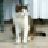
\includegraphics[height=1.5cm, align=c]{figures/carlini_wagner_orig.pdf} & 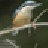
\includegraphics[height=1.5cm, align=c]{figures/carlini_wagner_adversarial.pdf} & 
\includegraphics[height=1.5cm, align=c]{figures/carlini_wagner_diff.pdf}\\
		\\
		Boundary & 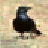
\includegraphics[height=1.5cm, align=c]{figures/boundary_orig.pdf} & 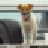
\includegraphics[height=1.5cm, align=c]{figures/boundary_adversarial.pdf} & 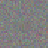
\includegraphics[height=1.5cm, align=c]{figures/boundary_diff.pdf}\\
		\\
		DeepFool & 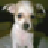
\includegraphics[height=1.5cm, align=c]{figures/deepfool_orig.pdf} & 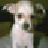
\includegraphics[height=1.5cm, align=c]{figures/deepfool_adversarial.pdf} & 
\includegraphics[height=1.5cm, align=c]{figures/deepfool_diff.pdf}\\
		\\
		Universal & 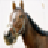
\includegraphics[height=1.5cm, align=c]{figures/universal_orig.pdf} & 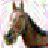
\includegraphics[height=1.5cm, align=c]{figures/universal_adversarial.pdf} & 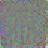
\includegraphics[height=1.5cm, align=c]{figures/universal_diff.pdf}\\
		\\
		\vspace{0.1cm}\\
	\end{tabular}
	\label{tab:images}
	\captionof{figure}{Original images from the CIFAR10 dataset (left), adversarial images (middle) and the corresponding perturbation (right) calculated for a CapsNet.}
\end{table}

Universal perturbations computed for CNNs transfer very well to CapsNets. Maby CapsNet universal perturbations don't work well, because we used FGSM? Maybe the loss is to blame. Would FGSM with cross entropy loss work on the CapsNet? Or FGSM with margin loss on CNN?
DeepFool actually seems to be a bit better for ConvNets. But the strong CW-attack fools both architecture with similarly small perturbations (Odd comparison, because CW is targeted. Maybe I should have used a untargeted CW version...)

\subsection{Visualizing Universal Perturbations}

We also visualized the universal perturbations calculated for the CapsNet and for the ConvNet using t-SNE \cite{tsne} and we observe that the perturbations for the CapsNet seem to be inherently different than the perturbations for the ConvNets.
\begin{figure}[h]
	\centering
	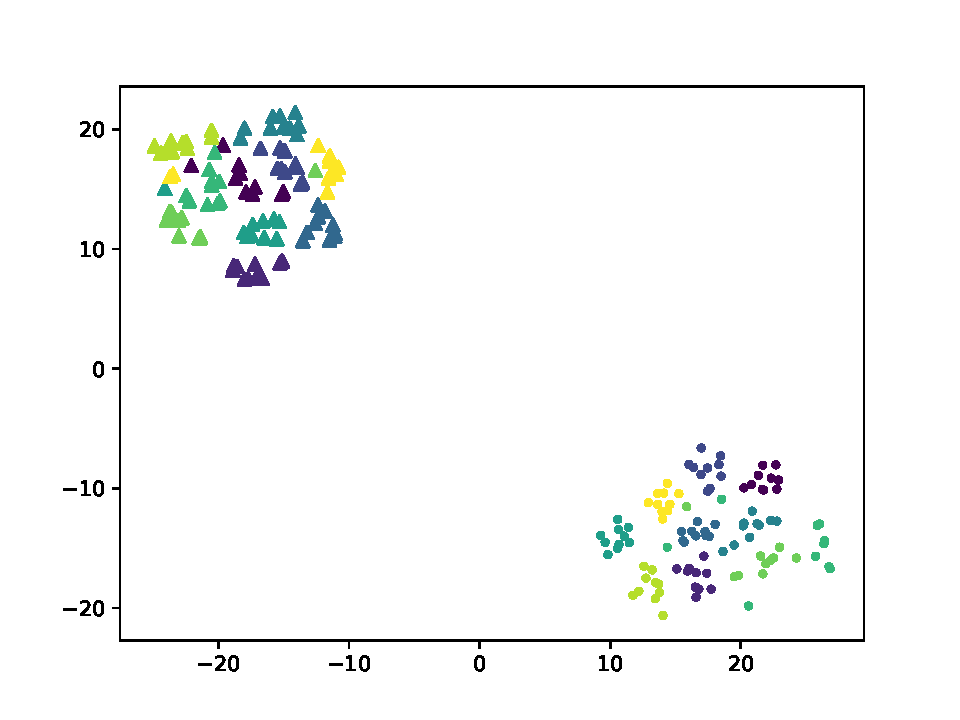
\includegraphics[height=5.5cm]{figures/tsne.pdf}
	\caption{Two dimensional embedding of the universal perturbations calculated using t-SNE \cite{tsne}. The upper right cluster represents perturbations calculated on a ConvNet, whereas the lower left cluster represents those calculated on a CapsNet. Perturbations with the same color were created using the same subset of test data.}
\end{figure}


\FloatBarrier
\section{Conclusion}
Our experiments show that CapsNets are not in general more robust to white-box attacks. With sufficiently sophisticated attacks CapsNets can be fooled as easily as ConvNets. 


% In the unusual situation where you want a paper to appear in the
% references without citing it in the main text, use \nocite
%\nocite{langley00}

\bibliography{icml}
\bibliographystyle{icml2019}



\end{document}


% This document was modified from the file originally made available by
% Pat Langley and Andrea Danyluk for ICML-2K. This version was created
% by Iain Murray in 2018, and modified by Alexandre Bouchard in
% 2019. Previous contributors include Dan Roy, Lise Getoor and Tobias
% Scheffer, which was slightly modified from the 2010 version by
% Thorsten Joachims & Johannes Fuernkranz, slightly modified from the
% 2009 version by Kiri Wagstaff and Sam Roweis's 2008 version, which is
% slightly modified from Prasad Tadepalli's 2007 version which is a
% lightly changed version of the previous year's version by Andrew
% Moore, which was in turn edited from those of Kristian Kersting and
% Codrina Lauth. Alex Smola contributed to the algorithmic style files.
